\section{Pinpointing single-link failures}

In this section we explain how to use a sr-cycle cover to detect single-link failures.

As mentioned in the introduction of this chapter, the idea is to have node $s$ 
regularly send monitoring probes over the sr-cycles of in a sr-cycle cover $C \subseteq \Csk$. Since we are using sr-cycles,
if the network is operating without failures, each probe must eventually come back to the vantage point $s$.
If at least one such probe does not come back, we know that at least one of the edges in the cycle associated with it
has a failure. We refer to the sr-cycles in the cycle cover $C$ as \emph{probing cycles}.

Let $\sr{c}$ be a cycle with a failure, that is, whose probe did not return. 
Because we use deterministic cycles, if we map $\sr{c}$ back to $G$, we get a cycle $c = (e_1, e_2, \ldots, e_l)$.
Recall that in this chapter we assume that the network $G$ is symmetric so that for each edge $e$ there is a reverse edge $\rev(e)$ and that
$\igp$ is symmetric if $\igp(e) = \rev(\igp(e))$.
The idea to detect the failure is to perform a binary search to find the largest $i$ such that
the cycle $c_i = (e_1, \ldots, e_i, \rev(e_i), \ldots, \rev(e_1))$ contains no failure. For each $i$ we send another 
probe over $c_i$ and check whether it comes back. If it does, then we know that the index we seek is greater than or equal to $i$. 
If it does not then the index must be strictly smaller than $i$. The single-link failure assumption is important for this process to work.
Because the probe did not cycle back, we know that one of 
$e_1, \ldots, e_l$ is faulty. Therefore, since we assume single-link
failure, we know that each reverse edge is not faulty. Hence, when we send a binary search probe on $c_i$, if it does not come back,
we know that the problem is in one of $e_1, \ldots, e_i$. We refer to these sr-cycles as \emph{identification cycles}.

Figure \ref{fig:bs-srcycle_new} illustrates this on an example with $l = 8$ and the failure is on edge $e_5$. We start the search with $i = 4$. The green dotted path
illustrates that the probe successfully returned to $v_1$. Thus we know that edges $e_1, e_2$ and $e_3$ are up.
The search will select $i = 6$ and this time the probe did not return. We conclude that the error is either in $e_4$ or $e_5$.
Finally, we send a probe on $c_5$ which returns. We finally conclude that the problem is on link $e_5$.

\begin{figure}
\begin{center}
\begin{tabular}{cc}
\begin{tikzpicture}[scale=0.75]
\node[scale=0.15] (a) at (3.000, 0.000) {\router{$v_1$}{router}};
\node[scale=0.15] (b) at (2.121, 2.121) {\router{$v_2$}{router}};
\node[scale=0.15] (c) at (0.000, 3.000) {\router{$v_3$}{router}};
\node[scale=0.15] (d) at (-2.121, 2.121) {\router{$v_4$}{router}};
\node[scale=0.15] (e) at (-3.000, 0.000) {\router{$v_5$}{router}};
\node[scale=0.15] (f) at (-2.121, -2.121) {\router{$v_6$}{router}};
\node[scale=0.15] (g) at (-0.000, -3.000) {\router{$v_7$}{router}};
\node[scale=0.15] (h) at (2.121, -2.121) {\router{$v_8$}{router}};

\draw[line width=2] (a) edge[above, sloped, bend right, ->] node[black,font=\bfseries] {\footnotesize \texttt{$e_1$}} (b);
\draw[line width=2] (b) edge[above, sloped, bend right, ->] node[black,font=\bfseries] {\footnotesize \texttt{$e_2$}} (c);
\draw[line width=2] (c) edge[above, sloped, bend right, ->] node[black,font=\bfseries] {\footnotesize \texttt{$e_3$}} (d);
\draw[line width=2] (d) edge[above, sloped, bend right, ->] node[black,font=\bfseries] {\footnotesize \texttt{$e_4$}} (e);
\draw[line width=2] (e) edge[below, sloped, bend right, ->] node[black,font=\bfseries] {\footnotesize \texttt{$e_5$}} (f);
\draw[line width=2] (f) edge[below, sloped, bend right, ->] node[black,font=\bfseries] {\footnotesize \texttt{$e_6$}} (g);
\draw[line width=2] (g) edge[below, sloped, bend right, ->] node[black,font=\bfseries] {\footnotesize \texttt{$e_7$}} (h);
\draw[line width=2] (h) edge[below, sloped, bend right, ->] node[black,font=\bfseries] {\footnotesize \texttt{$e_8$}} (a);
\draw (e) edge[sloped, bend right, ->] node[red, font=\bfseries] {\footnotesize \texttt{\Large \textsf{X}}} (f);

\draw[line width=2, gray] (a) edge[below, sloped, bend left, <-] node[gray,font=\bfseries] {\footnotesize \texttt{$\rev(e_1)$}} (b);
\draw[line width=2, gray] (b) edge[below, sloped, bend left, <-] node[gray,font=\bfseries] {\footnotesize \texttt{$\rev(e_2)$}} (c);
\draw[line width=2, gray] (c) edge[below, sloped, bend left, <-] node[gray,font=\bfseries] {\footnotesize \texttt{$\rev(e_3)$}} (d);
\draw[line width=2, gray] (d) edge[below, sloped, bend left, <-] node[gray,font=\bfseries] {\footnotesize \texttt{$\rev(e_4)$}} (e);
\draw[line width=2, gray] (e) edge[above, sloped, bend left, <-] node[gray,font=\bfseries] {\footnotesize \texttt{$\rev(e_5)$}} (f);

\draw[line width=2, gray] (f) edge[above, sloped, bend left, <-] node[gray,font=\bfseries] {\footnotesize \texttt{$\rev(e_6)$}} (g);
\draw[line width=2, gray] (g) edge[above, sloped, bend left, <-] node[gray,font=\bfseries] {\footnotesize \texttt{$\rev(e_7)$}} (h);
\draw[line width=2, gray] (h) edge[above, sloped, bend left, <-] node[gray,font=\bfseries] {\footnotesize \texttt{$\rev(e_8)$}} (a);

\draw[darkgreen, ultra thick, dotted, ->] plot [smooth] coordinates { ($(a)+(0.5,0)$) ($(b)+(0,0.5)$) ($(c)+(0,0.5)$) ($(d)+(0,0.5)$) ($(d)+(-0.5,0)$) ($(d)+(0,-0.5)$) ($(c)+(0,-0.5)$) ($(b)+(0,-0.5)$) ($(a)$) };

\end{tikzpicture}

&

\begin{tikzpicture}[scale=0.75]
\node[scale=0.15] (1) at (3.000, 0.000) {\router{$v_1$}{router}};
\node[scale=0.15] (2) at (2.121, 2.121) {\router{$v_2$}{router}};
\node[scale=0.15] (3) at (0.000, 3.000) {\router{$v_3$}{router}};
\node[scale=0.15] (4) at (-2.121, 2.121) {\router{$v_4$}{green}};
\node[scale=0.15] (5) at (-3.000, 0.000) {\router{$v_5$}{router}};
\node[scale=0.15] (6) at (-2.121, -2.121) {\router{$v_6$}{router}};
\node[scale=0.15] (7) at (-0.000, -3.000) {\router{$v_7$}{router}};
\node[scale=0.15] (8) at (2.121, -2.121) {\router{$v_8$}{router}};

\draw[line width=2, darkgreen] (1) edge[above, sloped, bend right, ->] node[black,font=\bfseries] {\footnotesize \texttt{$e_1$}} (2);
\draw[line width=2, darkgreen] (2) edge[above, sloped, bend right, ->] node[black,font=\bfseries] {\footnotesize \texttt{$e_2$}} (3);
\draw[line width=2, darkgreen] (3) edge[above, sloped, bend right, ->] node[black,font=\bfseries] {\footnotesize \texttt{$e_3$}} (4);
\draw[line width=2] (4) edge[above, sloped, bend right, ->] node[black,font=\bfseries] {\footnotesize \texttt{$e_4$}} (5);
\draw[line width=2] (5) edge[below, sloped, bend right, ->] node[black,font=\bfseries] {\footnotesize \texttt{$e_5$}} (6);
\draw[line width=2] (6) edge[below, sloped, bend right, ->] node[black,font=\bfseries] {\footnotesize \texttt{$e_6$}} (7);
\draw[line width=2] (7) edge[below, sloped, bend right, ->] node[black,font=\bfseries] {\footnotesize \texttt{$e_7$}} (8);
\draw[line width=2] (8) edge[below, sloped, bend right, ->] node[black,font=\bfseries] {\footnotesize \texttt{$e_8$}} (1);
\draw (5) edge[sloped, bend right, ->] node[red, font=\bfseries] {\footnotesize \texttt{\Large \textsf{X}}} (6);

\draw[line width=2, gray, darkgreen] (1) edge[below, sloped, bend left, <-] node[gray,font=\bfseries] {\footnotesize \texttt{$\rev(e_1)$}} (2);
\draw[line width=2, gray, darkgreen] (2) edge[below, sloped, bend left, <-] node[gray,font=\bfseries] {\footnotesize \texttt{$\rev(e_2)$}} (3);
\draw[line width=2, gray, darkgreen] (3) edge[below, sloped, bend left, <-] node[gray,font=\bfseries] {\footnotesize \texttt{$\rev(e_3)$}} (4);
\draw[line width=2, gray] (4) edge[below, sloped, bend left, <-] node[gray,font=\bfseries] {\footnotesize \texttt{$\rev(e_4)$}} (5);
\draw[line width=2, gray] (5) edge[above, sloped, bend left, <-] node[gray,font=\bfseries] {\footnotesize \texttt{$\rev(e_5)$}} (6);
\draw[line width=2, gray] (6) edge[above, sloped, bend left, <-] node[gray,font=\bfseries] {\footnotesize \texttt{$\rev(e_6)$}} (7);
\draw[line width=2, gray] (7) edge[above, sloped, bend left, <-] node[gray,font=\bfseries] {\footnotesize \texttt{$\rev(e_7)$}} (8);
\draw[line width=2, gray] (8) edge[above, sloped, bend left, <-] node[gray,font=\bfseries] {\footnotesize \texttt{$\rev(e_8)$}} (1);

\draw[red!50!black, ultra thick, dotted, ->] plot [smooth] coordinates { 
($(a)+(0.5,0)$) ($(b)+(0,0.5)$) ($(c)+(0,0.5)$) ($(d)+(0,0.5)$) ($(e)+(-0.5,0)$) ($(f)+(-0.5,0)$) 
($(f)+(0,-0.5)$) ($(f)+(0.5,0)$) ($(e)+(0.5,0)$) ($(d)+(0,-0.5)$) ($(c)+(0,-0.5)$) ($(b)+(0,-0.5)$) ($(a)$) 
};

\end{tikzpicture}

\\

\footnotesize

First step of binary search. Success.

&

\footnotesize

Second step of binary search. Failure.

\\

\footnotesize

Edges $e_1, e_2, e_3$ are up.

&

\footnotesize

One of $e_4, e_5$ is down.

\\[0.5cm]

\begin{tikzpicture}[scale=0.75]
\node[scale=0.15] (1) at (3.000, 0.000) {\router{$v_1$}{router}};
\node[scale=0.15] (2) at (2.121, 2.121) {\router{$v_2$}{router}};
\node[scale=0.15] (3) at (0.000, 3.000) {\router{$v_3$}{router}};
\node[scale=0.15] (4) at (-2.121, 2.121) {\router{$v_4$}{green}};
\node[scale=0.15] (5) at (-3.000, 0.000) {\router{$v_5$}{router}};
\node[scale=0.15] (6) at (-2.121, -2.121) {\router{$v_6$}{red!50!white}};
\node[scale=0.15] (7) at (-0.000, -3.000) {\router{$v_7$}{router}};
\node[scale=0.15] (8) at (2.121, -2.121) {\router{$v_8$}{router}};

\draw[line width=2, darkgreen] (1) edge[above, sloped, bend right, ->] node[black,font=\bfseries] {\footnotesize \texttt{$e_1$}} (2);
\draw[line width=2, darkgreen] (2) edge[above, sloped, bend right, ->] node[black,font=\bfseries] {\footnotesize \texttt{$e_2$}} (3);
\draw[line width=2, darkgreen] (3) edge[above, sloped, bend right, ->] node[black,font=\bfseries] {\footnotesize \texttt{$e_3$}} (4);
\draw[line width=2] (4) edge[above, sloped, bend right, ->] node[black,font=\bfseries] {\footnotesize \texttt{$e_4$}} (5);
\draw[line width=2] (5) edge[below, sloped, bend right, ->] node[black,font=\bfseries] {\footnotesize \texttt{$e_5$}} (6);
\draw[line width=2] (6) edge[below, sloped, bend right, ->] node[black,font=\bfseries] {\footnotesize \texttt{$e_6$}} (7);
\draw[line width=2] (7) edge[below, sloped, bend right, ->] node[black,font=\bfseries] {\footnotesize \texttt{$e_7$}} (8);
\draw[line width=2] (8) edge[below, sloped, bend right, ->] node[black,font=\bfseries] {\footnotesize \texttt{$e_8$}} (1);
\draw (5) edge[sloped, bend right, ->] node[red, font=\bfseries] {\footnotesize \texttt{\Large \textsf{X}}} (6);

\draw[line width=2, gray, darkgreen] (1) edge[below, sloped, bend left, <-] node[gray,font=\bfseries] {\footnotesize \texttt{$\rev(e_1)$}} (2);
\draw[line width=2, gray, darkgreen] (2) edge[below, sloped, bend left, <-] node[gray,font=\bfseries] {\footnotesize \texttt{$\rev(e_2)$}} (3);
\draw[line width=2, gray, darkgreen] (3) edge[below, sloped, bend left, <-] node[gray,font=\bfseries] {\footnotesize \texttt{$\rev(e_3)$}} (4);
\draw[line width=2, gray] (4) edge[below, sloped, bend left, <-] node[gray,font=\bfseries] {\footnotesize \texttt{$\rev(e_4)$}} (5);
\draw[line width=2, gray] (5) edge[above, sloped, bend left, <-] node[gray,font=\bfseries] {\footnotesize \texttt{$\rev(e_5)$}} (6);
\draw[line width=2, gray] (6) edge[above, sloped, bend left, <-] node[gray,font=\bfseries] {\footnotesize \texttt{$\rev(e_6)$}} (7);
\draw[line width=2, gray] (7) edge[above, sloped, bend left, <-] node[gray,font=\bfseries] {\footnotesize \texttt{$\rev(e_7)$}} (8);
\draw[line width=2, gray] (8) edge[above, sloped, bend left, <-] node[gray,font=\bfseries] {\footnotesize \texttt{$\rev(e_8)$}} (1);

\draw[darkgreen, ultra thick, dotted, ->] plot [smooth] coordinates { 
($(a)+(0.5,0)$) ($(b)+(0,0.5)$) ($(c)+(0,0.5)$) ($(d)+(0,0.5)$) ($(e)+(-0.5,0)$) 
($(e)+(0,-0.5)$) ($(e)+(0.5,0)$) ($(d)+(0,-0.5)$) ($(c)+(0,-0.5)$) ($(b)+(0,-0.5)$) ($(a)$) 
};

\end{tikzpicture}

&


\begin{tikzpicture}[scale=0.75]
\node[scale=0.15] (1) at (3.000, 0.000) {\router{$v_1$}{router}};
\node[scale=0.15] (2) at (2.121, 2.121) {\router{$v_2$}{router}};
\node[scale=0.15] (3) at (0.000, 3.000) {\router{$v_3$}{router}};
\node[scale=0.15] (4) at (-2.121, 2.121) {\router{$v_4$}{green}};
\node[scale=0.15] (5) at (-3.000, 0.000) {\router{$v_5$}{green}};
\node[scale=0.15] (6) at (-2.121, -2.121) {\router{$v_6$}{red!50!white}};
\node[scale=0.15] (7) at (-0.000, -3.000) {\router{$v_7$}{router}};
\node[scale=0.15] (8) at (2.121, -2.121) {\router{$v_8$}{router}};

\draw[line width=2, darkgreen] (1) edge[above, sloped, bend right, ->] node[black,font=\bfseries] {\footnotesize \texttt{$e_1$}} (2);
\draw[line width=2, darkgreen] (2) edge[above, sloped, bend right, ->] node[black,font=\bfseries] {\footnotesize \texttt{$e_2$}} (3);
\draw[line width=2, darkgreen] (3) edge[above, sloped, bend right, ->] node[black,font=\bfseries] {\footnotesize \texttt{$e_3$}} (4);
\draw[line width=2, darkgreen] (4) edge[above, sloped, bend right, ->] node[black,font=\bfseries] {\footnotesize \texttt{$e_4$}} (5);
\draw[line width=2] (5) edge[below, red!50!black, sloped, bend right, ->] node[black,font=\bfseries] {\footnotesize \texttt{$e_5$}} (6);
\draw[line width=2, opacity=0] (5) edge[red!50!black, sloped, bend right, ->] node (e5) {} (6);
\draw (5) edge[sloped, bend right, ->] node[red, font=\bfseries] {\footnotesize \texttt{\Large \textsf{X}}} (6);

\draw[line width=2] (6) edge[below, sloped, bend right, ->] node[black,font=\bfseries] {\footnotesize \texttt{$e_6$}} (7);
\draw[line width=2] (7) edge[below, sloped, bend right, ->] node[black,font=\bfseries] {\footnotesize \texttt{$e_7$}} (8);
\draw[line width=2] (8) edge[below, sloped, bend right, ->] node[black,font=\bfseries] {\footnotesize \texttt{$e_8$}} (1);

\draw[line width=2, gray, darkgreen] (1) edge[below, sloped, bend left, <-] node[gray,font=\bfseries] {\footnotesize \texttt{$\rev(e_1)$}} (2);
\draw[line width=2, gray, darkgreen] (2) edge[below, sloped, bend left, <-] node[gray,font=\bfseries] {\footnotesize \texttt{$\rev(e_2)$}} (3);
\draw[line width=2, gray, darkgreen] (3) edge[below, sloped, bend left, <-] node[gray,font=\bfseries] {\footnotesize \texttt{$\rev(e_3)$}} (4);
\draw[line width=2, gray, darkgreen] (4) edge[below, sloped, bend left, <-] node[gray,font=\bfseries] {\footnotesize \texttt{$\rev(e_4)$}} (5);
\draw[line width=2, gray, gray] (5) edge[above, sloped, bend left, <-] node[gray,font=\bfseries] {\footnotesize \texttt{$\rev(e_5)$}} (6);
%\draw[line width=2, gray, red!50!black, opacity=0] (5) edge[sloped, bend left, <-] node[gray,font=\bfseries] (re5) {} (6);


\draw[line width=2, gray] (6) edge[above, sloped, bend left, <-] node[gray,font=\bfseries] {\footnotesize \texttt{$\rev(e_6)$}} (7);
\draw[line width=2, gray] (7) edge[above, sloped, bend left, <-] node[gray,font=\bfseries] {\footnotesize \texttt{$\rev(e_7)$}} (8);
\draw[line width=2, gray] (8) edge[above, sloped, bend left, <-] node[gray,font=\bfseries] {\footnotesize \texttt{$\rev(e_8)$}} (1);

%\draw[darkgreen, ultra thick, dotted, ->] plot [smooth] coordinates { 
%($(a)+(0.5,0)$) ($(b)+(0,0.5)$) ($(c)+(0,0.5)$) ($(d)+(0,0.5)$) ($(e)+(-0.5,0)$) 
%($(e)+(0,-0.5)$) ($(e)+(0.5,0)$) ($(d)+(0,-0.5)$) ($(c)+(0,-0.5)$) ($(b)+(0,-0.5)$) ($(a)$) 
%};

%\node (fail) at (0, 0) {failure};

%\draw[->, dashed] (fail) -- (e5);
%\draw[->, dashed] (fail) -- (re5);


\end{tikzpicture}

\\

\footnotesize

Third step of binary search. Success.

&

\footnotesize

End of the search.

\\

\footnotesize

Edges $e_4$ is up.

&

\footnotesize

Failure detected in $e_5$.

\end{tabular}
\end{center}
\caption{Binary search to identify the failure (single-link failure assumption).}
\label{fig:bs-srcycle_new}
\end{figure}

To illustrate why the single link-failure assumption is important, let's see happens with this process
when multiple failures occur. Imagine the same example as in Figure \ref{fig:bs-srcycle_new} but assume that
edge $\rev(e_3)$ is also down. In this case the first binary search probe will fail to return and the search
will stop at $i = 3$ and the algorithm will say that the problem is on edge $e_3$. However $e_3$ is up
and it is $\rev(e_3)$ that prevents the probe to return. This shows that with multiple failures, we cannot
know exactly which link is down. However, we still can say that either $e_3$ is down \emph{or} $\rev(e_3)$ is
down. Figure \ref{fig:bs-srcycle_new2} illustrates this.

This means that in presence of multiple link failures, we cannot tell exactly which link is down but we can
still find a set of two links $\{ e, \rev(e) \}$ such that we are sure that at least one of them is down.

\begin{figure}
\begin{center}
\begin{tabular}{cc}
\begin{tikzpicture}[scale=0.75]
\node[scale=0.15] (a) at (3.000, 0.000) {\router{$v_1$}{router}};
\node[scale=0.15] (b) at (2.121, 2.121) {\router{$v_2$}{router}};
\node[scale=0.15] (c) at (0.000, 3.000) {\router{$v_3$}{router}};
\node[scale=0.15] (d) at (-2.121, 2.121) {\router{$v_4$}{router}};
\node[scale=0.15] (e) at (-3.000, 0.000) {\router{$v_5$}{router}};
\node[scale=0.15] (f) at (-2.121, -2.121) {\router{$v_6$}{router}};
\node[scale=0.15] (g) at (-0.000, -3.000) {\router{$v_7$}{router}};
\node[scale=0.15] (h) at (2.121, -2.121) {\router{$v_8$}{router}};

\draw[line width=2] (a) edge[above, sloped, bend right, ->] node[black,font=\bfseries] {\footnotesize \texttt{$e_1$}} (b);
\draw[line width=2] (b) edge[above, sloped, bend right, ->] node[black,font=\bfseries] {\footnotesize \texttt{$e_2$}} (c);
\draw[line width=2] (c) edge[above, sloped, bend right, ->] node[black,font=\bfseries] {\footnotesize \texttt{$e_3$}} (d);
\draw[line width=2] (d) edge[above, sloped, bend right, ->] node[black,font=\bfseries] {\footnotesize \texttt{$e_4$}} (e);
\draw[line width=2] (e) edge[below, sloped, bend right, ->] node[black,font=\bfseries] {\footnotesize \texttt{$e_5$}} (f);
\draw[line width=2] (f) edge[below, sloped, bend right, ->] node[black,font=\bfseries] {\footnotesize \texttt{$e_6$}} (g);
\draw[line width=2] (g) edge[below, sloped, bend right, ->] node[black,font=\bfseries] {\footnotesize \texttt{$e_7$}} (h);
\draw[line width=2] (h) edge[below, sloped, bend right, ->] node[black,font=\bfseries] {\footnotesize \texttt{$e_8$}} (a);
\draw (e) edge[sloped, bend right, ->] node[red, font=\bfseries] {\Large \textsf{X}} (f);

\draw[line width=2, gray] (a) edge[below, sloped, bend left, <-] node[gray,font=\bfseries] {\footnotesize \texttt{$\rev(e_1)$}} (b);
\draw[line width=2, gray] (b) edge[below, sloped, bend left, <-] node[gray,font=\bfseries] {\footnotesize \texttt{$\rev(e_2)$}} (c);
\draw[line width=2, gray] (c) edge[below, sloped, bend left, <-] node[gray,font=\bfseries] {\footnotesize \texttt{$\rev(e_3)$}} (d);
\draw[line width=2, gray] (d) edge[below, sloped, bend left, <-] node[gray,font=\bfseries] {\footnotesize \texttt{$\rev(e_4)$}} (e);
\draw[line width=2, gray] (e) edge[above, sloped, bend left, <-] node[gray,font=\bfseries] {\footnotesize \texttt{$\rev(e_5)$}} (f);
\draw[line width=2, gray] (c) edge[sloped, bend left, <-] node[red,font=\bfseries] {\Large \textsf{X}} (d);

\draw[line width=2, gray] (f) edge[above, sloped, bend left, <-] node[gray,font=\bfseries] {\footnotesize \texttt{$\rev(e_6)$}} (g);
\draw[line width=2, gray] (g) edge[above, sloped, bend left, <-] node[gray,font=\bfseries] {\footnotesize \texttt{$\rev(e_7)$}} (h);
\draw[line width=2, gray] (h) edge[above, sloped, bend left, <-] node[gray,font=\bfseries] {\footnotesize \texttt{$\rev(e_8)$}} (a);

\draw[red!50!black, ultra thick, dotted, ->] plot [smooth] coordinates { ($(a)+(0.5,0)$) ($(b)+(0,0.5)$) ($(c)+(0,0.5)$) ($(d)+(0,0.5)$) ($(d)+(-0.5,0)$) ($(d)+(0,-0.5)$) ($(c)+(0,-0.5)$) ($(b)+(0,-0.5)$) ($(a)$) };

\end{tikzpicture}

&

\begin{tikzpicture}[scale=0.75]
\node[scale=0.15] (1) at (3.000, 0.000) {\router{$v_1$}{router}};
\node[scale=0.15] (2) at (2.121, 2.121) {\router{$v_2$}{router}};
\node[scale=0.15] (3) at (0.000, 3.000) {\router{$v_3$}{router}};
\node[scale=0.15] (4) at (-2.121, 2.121) {\router{$v_4$}{red!50!white}};
\node[scale=0.15] (5) at (-3.000, 0.000) {\router{$v_5$}{router}};
\node[scale=0.15] (6) at (-2.121, -2.121) {\router{$v_6$}{router}};
\node[scale=0.15] (7) at (-0.000, -3.000) {\router{$v_7$}{router}};
\node[scale=0.15] (8) at (2.121, -2.121) {\router{$v_8$}{router}};

\draw[line width=2] (1) edge[above, sloped, bend right, ->] node[black,font=\bfseries] {\footnotesize \texttt{$e_1$}} (2);
\draw[line width=2] (2) edge[above, sloped, bend right, ->] node[black,font=\bfseries] {\footnotesize \texttt{$e_2$}} (3);
\draw[line width=2] (3) edge[above, sloped, bend right, ->] node[black,font=\bfseries] {\footnotesize \texttt{$e_3$}} (4);
\draw[line width=2] (4) edge[above, sloped, bend right, ->] node[black,font=\bfseries] {\footnotesize \texttt{$e_4$}} (5);
\draw[line width=2] (5) edge[below, sloped, bend right, ->] node[black,font=\bfseries] {\footnotesize \texttt{$e_5$}} (6);
\draw[line width=2] (6) edge[below, sloped, bend right, ->] node[black,font=\bfseries] {\footnotesize \texttt{$e_6$}} (7);
\draw[line width=2] (7) edge[below, sloped, bend right, ->] node[black,font=\bfseries] {\footnotesize \texttt{$e_7$}} (8);
\draw[line width=2] (8) edge[below, sloped, bend right, ->] node[black,font=\bfseries] {\footnotesize \texttt{$e_8$}} (1);
\draw (5) edge[sloped, bend right, ->] node[red, font=\bfseries] {\footnotesize \texttt{\Large \textsf{X}}} (6);

\draw[line width=2, gray] (1) edge[below, sloped, bend left, <-] node[gray,font=\bfseries] {\footnotesize \texttt{$\rev(e_1)$}} (2);
\draw[line width=2, gray] (2) edge[below, sloped, bend left, <-] node[gray,font=\bfseries] {\footnotesize \texttt{$\rev(e_2)$}} (3);
\draw[line width=2, gray] (3) edge[below, sloped, bend left, <-] node[gray,font=\bfseries] {\footnotesize \texttt{$\rev(e_3)$}} (4);
\draw[line width=2, gray] (4) edge[below, sloped, bend left, <-] node[gray,font=\bfseries] {\footnotesize \texttt{$\rev(e_4)$}} (5);
\draw[line width=2, gray] (5) edge[above, sloped, bend left, <-] node[gray,font=\bfseries] {\footnotesize \texttt{$\rev(e_5)$}} (6);
\draw[line width=2, gray] (6) edge[above, sloped, bend left, <-] node[gray,font=\bfseries] {\footnotesize \texttt{$\rev(e_6)$}} (7);
\draw[line width=2, gray] (7) edge[above, sloped, bend left, <-] node[gray,font=\bfseries] {\footnotesize \texttt{$\rev(e_7)$}} (8);
\draw[line width=2, gray] (8) edge[above, sloped, bend left, <-] node[gray,font=\bfseries] {\footnotesize \texttt{$\rev(e_8)$}} (1);
\draw[line width=2, gray] (c) edge[sloped, bend left, <-] node[red,font=\bfseries] {\Large \textsf{X}} (d);

\draw[darkgreen, ultra thick, dotted, ->] plot [smooth] coordinates 
{ ($(a)+(0.5,0)$) ($(b)+(0.5,0.5)$) ($(b)+(0,0.5)$) ($(b)+(-0.5,0)$)($(a)$) };

\end{tikzpicture}

\\

\footnotesize

First step of binary search. Failure.

&

\footnotesize

Second step of binary search. Success.

\\

\footnotesize

One of $e_1, e_2, e_3, \rev(e_3), \rev(e_2), \rev(e_1)$ is down.

&

\footnotesize

Edges $e_1, \rev(e_1)$ are up.

\\[0.5cm]

\begin{tikzpicture}[scale=0.75]
\node[scale=0.15] (1) at (3.000, 0.000) {\router{$v_1$}{router}};
\node[scale=0.15] (2) at (2.121, 2.121) {\router{$v_2$}{green}};
\node[scale=0.15] (3) at (0.000, 3.000) {\router{$v_3$}{router}};
\node[scale=0.15] (4) at (-2.121, 2.121) {\router{$v_4$}{red!50!white}};
\node[scale=0.15] (5) at (-3.000, 0.000) {\router{$v_5$}{router}};
\node[scale=0.15] (6) at (-2.121, -2.121) {\router{$v_6$}{router}};
\node[scale=0.15] (7) at (-0.000, -3.000) {\router{$v_7$}{router}};
\node[scale=0.15] (8) at (2.121, -2.121) {\router{$v_8$}{router}};

\draw[line width=2] (1) edge[darkgreen, sloped, bend right, ->] node[black,font=\bfseries] {\footnotesize \texttt{$e_1$}} (2);
\draw[line width=2] (2) edge[above, sloped, bend right, ->] node[black,font=\bfseries] {\footnotesize \texttt{$e_2$}} (3);
\draw[line width=2] (3) edge[above, sloped, bend right, ->] node[black,font=\bfseries] {\footnotesize \texttt{$e_3$}} (4);
\draw[line width=2] (4) edge[above, sloped, bend right, ->] node[black,font=\bfseries] {\footnotesize \texttt{$e_4$}} (5);
\draw[line width=2] (5) edge[below, sloped, bend right, ->] node[black,font=\bfseries] {\footnotesize \texttt{$e_5$}} (6);
\draw[line width=2] (6) edge[below, sloped, bend right, ->] node[black,font=\bfseries] {\footnotesize \texttt{$e_6$}} (7);
\draw[line width=2] (7) edge[below, sloped, bend right, ->] node[black,font=\bfseries] {\footnotesize \texttt{$e_7$}} (8);
\draw[line width=2] (8) edge[below, sloped, bend right, ->] node[black,font=\bfseries] {\footnotesize \texttt{$e_8$}} (1);
\draw (5) edge[sloped, bend right, ->] node[red, font=\bfseries] {\footnotesize \texttt{\Large \textsf{X}}} (6);

\draw[line width=2, gray] (1) edge[darkgreen, below, sloped, bend left, <-] node[gray,font=\bfseries] {\footnotesize \texttt{$\rev(e_1)$}} (2);
\draw[line width=2, gray] (2) edge[below, sloped, bend left, <-] node[gray,font=\bfseries] {\footnotesize \texttt{$\rev(e_2)$}} (3);
\draw[line width=2, gray] (3) edge[below, sloped, bend left, <-] node[gray,font=\bfseries] {\footnotesize \texttt{$\rev(e_3)$}} (4);
\draw[line width=2, gray] (4) edge[below, sloped, bend left, <-] node[gray,font=\bfseries] {\footnotesize \texttt{$\rev(e_4)$}} (5);
\draw[line width=2, gray] (5) edge[above, sloped, bend left, <-] node[gray,font=\bfseries] {\footnotesize \texttt{$\rev(e_5)$}} (6);
\draw[line width=2, gray] (6) edge[above, sloped, bend left, <-] node[gray,font=\bfseries] {\footnotesize \texttt{$\rev(e_6)$}} (7);
\draw[line width=2, gray] (7) edge[above, sloped, bend left, <-] node[gray,font=\bfseries] {\footnotesize \texttt{$\rev(e_7)$}} (8);
\draw[line width=2, gray] (8) edge[above, sloped, bend left, <-] node[gray,font=\bfseries] {\footnotesize \texttt{$\rev(e_8)$}} (1);
\draw[line width=2, gray] (c) edge[sloped, bend left, <-] node[red,font=\bfseries] {\Large \textsf{X}} (d);

\draw[darkgreen, ultra thick, dotted, ->] plot [smooth] coordinates 
{ ($(a)+(0.5,0)$) ($(b)+(0,0.5)$) ($(c)+(0,0.5)$) ($(c)+(-0.5,0)$) ($(c)+(0,-0.5)$) ($(b)+(0,-0.5)$) ($(a)$) };

\end{tikzpicture}


&


\begin{tikzpicture}[scale=0.75]
\node[scale=0.15] (1) at (3.000, 0.000) {\router{$v_1$}{router}};
\node[scale=0.15] (2) at (2.121, 2.121) {\router{$v_2$}{green}};
\node[scale=0.15] (3) at (0.000, 3.000) {\router{$v_3$}{green}};
\node[scale=0.15] (4) at (-2.121, 2.121) {\router{$v_4$}{red!50!white}};
\node[scale=0.15] (5) at (-3.000, 0.000) {\router{$v_5$}{router}};
\node[scale=0.15] (6) at (-2.121, -2.121) {\router{$v_6$}{router}};
\node[scale=0.15] (7) at (-0.000, -3.000) {\router{$v_7$}{router}};
\node[scale=0.15] (8) at (2.121, -2.121) {\router{$v_8$}{router}};

\draw[line width=2, darkgreen] (1) edge[darkgreen,above, sloped, bend right, ->] node[black,font=\bfseries] {\footnotesize \texttt{$e_1$}} (2);
\draw[line width=2, darkgreen] (2) edge[darkgreen,above, sloped, bend right, ->] node[black,font=\bfseries] {\footnotesize \texttt{$e_2$}} (3);
\draw[line width=2, red!50!black] (3) edge[above, sloped, bend right, ->] node[black,font=\bfseries] {\footnotesize \texttt{$e_3$}} (4);
\draw[line width=2] (4) edge[above, sloped, bend right, ->] node[black,font=\bfseries] {\footnotesize \texttt{$e_4$}} (5);
\draw[line width=2] (5) edge[below, sloped, bend right, ->] node[black,font=\bfseries] {\footnotesize \texttt{$e_5$}} (6);
%\draw[line width=2] (3) edge[sloped, bend right, ->] node (e3) {} (4);
\draw (5) edge[sloped, bend right, ->] node[red, font=\bfseries] {\footnotesize \texttt{\Large \textsf{X}}} (6);

\draw[line width=2] (6) edge[below, sloped, bend right, ->] node[black,font=\bfseries] {\footnotesize \texttt{$e_6$}} (7);
\draw[line width=2] (7) edge[below, sloped, bend right, ->] node[black,font=\bfseries] {\footnotesize \texttt{$e_7$}} (8);
\draw[line width=2] (8) edge[below, sloped, bend right, ->] node[black,font=\bfseries] {\footnotesize \texttt{$e_8$}} (1);

\draw[line width=2, gray, darkgreen] (1) edge[darkgreen,below, sloped, bend left, <-] node[gray,font=\bfseries] {\footnotesize \texttt{$\rev(e_1)$}} (2);
\draw[line width=2, gray, darkgreen] (2) edge[darkgreen,below, sloped, bend left, <-] node[gray,font=\bfseries] {\footnotesize \texttt{$\rev(e_2)$}} (3);

\draw[line width=2, red!50!black] (3) edge[below, sloped, bend left, <-] node[gray,font=\bfseries] {\footnotesize \texttt{$\rev(e_3)$}} (4);

\draw[line width=2, gray] (4) edge[below, sloped, bend left, <-] node[gray,font=\bfseries] {\footnotesize \texttt{$\rev(e_4)$}} (5);
\draw[line width=2, gray, gray] (5) edge[above, sloped, bend left, <-] node[gray,font=\bfseries] {\footnotesize \texttt{$\rev(e_5)$}} (6);
%\draw[line width=2, gray, opacity=0] (3) edge[sloped, bend left, <-] node[gray,font=\bfseries] (re5) {} (4);

\draw[line width=2, red!50!black] (c) edge[sloped, bend left, <-] node[red,font=\bfseries] {\Large \textsf{X}} (d);

\draw[line width=2, gray] (6) edge[above, sloped, bend left, <-] node[gray,font=\bfseries] {\footnotesize \texttt{$\rev(e_6)$}} (7);
\draw[line width=2, gray] (7) edge[above, sloped, bend left, <-] node[gray,font=\bfseries] {\footnotesize \texttt{$\rev(e_7)$}} (8);
\draw[line width=2, gray] (8) edge[above, sloped, bend left, <-] node[gray,font=\bfseries] {\footnotesize \texttt{$\rev(e_8)$}} (1);

%\draw[darkgreen, ultra thick, dotted, ->] plot [smooth] coordinates { 
%($(a)+(0.5,0)$) ($(b)+(0,0.5)$) ($(c)+(0,0.5)$) ($(d)+(0,0.5)$) ($(e)+(-0.5,0)$) 
%($(e)+(0,-0.5)$) ($(e)+(0.5,0)$) ($(d)+(0,-0.5)$) ($(c)+(0,-0.5)$) ($(b)+(0,-0.5)$) ($(a)$) 
%};


\end{tikzpicture}

\\

\footnotesize

Third step of binary search. Success.

&

\footnotesize

End of the search.

\\

\footnotesize

Edges $e_2, \rev(e_2)$ are up.

&

\footnotesize

Failure in $e_3$ or $\rev(e_3)$.

\end{tabular}
\end{center}
\caption{Binary search to identify the failure. No single-link failure assumption.}
\label{fig:bs-srcycle_new2}
\end{figure}

\subsubsection*{Computing identification cycles}

At each step of the binary search, given $i$ we need to find a way to route a probe over the cycle
$c_i = (e_1, \ldots, e_{i - 1}, e_i, \rev(e_i), \rev(e_{i - 1}), \ldots, \rev(e_1))$. One way do so
is to compute a minimum segmentation of $c_i$ and use that segmentation. 

There is an alternative solution that avoids having to compute segmentations and uses the segments
in $\sr{c} = \langle x_1, \ldots, x_l \rangle$ instead to segment the identification cycles. We will do so by finding an index $i$ such that
$e_i$ is between $x_j$ and $x_{j + 1}$ and then reverse the elements $x_1, \ldots, x_j$
to obtain a segmentation of $c_i = (e_1, \ldots, e_{i - 1}, e_i, \rev(e_i), \rev(e_{i - 1}), \ldots, \rev(e_1))$.

\begin{definition}
Let $G$ be a symmetric network and $\sr{p}$ be a sr-path on $G$. We define $\rev(\sr{p}) = \langle \rev(x_l) \ldots, \rev(x_1) \rangle$ where
$\rev(x_i) = x_i$ if $x_i \in V(G)$ and $\rev(x_i) = \rev(e)$ if $x_i = e \in E(G)$.

Note that we have $\rev(x_i)^1 = x^2_i$ and $\rev(x_i)^2 = x^1_i$.
\end{definition}

\begin{lemma}
\label{lemma:rev-sr}
Let $G$ be a symmetric network. Let $\sr{p}$ be a deterministic sr-path
with $\seq(\sr{p}) = (e_1, \ldots, e_n)$. If $\igp$ is symmetric then $\rev(\sr{p})$ is a deterministic sr-path with 
$\seq(\rev(\sr{p})) = (\rev(e_n), \ldots, \rev(e_1)) = \rev(\seq(\sr{p}))$.
\end{lemma}

\begin{proof}
We first prove that $\rev(\sr{p})$ is deterministic. Let $i \in \{l, \ldots, 2\}$. We need to prove that there 
is a unique shortest path from $\rev(x_i)^2 = x^1_i$ to $\rev(x_{i - 1})^1 = x^2_{i - 1}$. Since $\sr{p}$
is deterministic, we know that there is a unique shortest path from $x^2_{i - 1}$ to $x^1_i$. By Corollary 
\ref{cor:dag-rev} we know then that there is also a unique shortest path from $x^1_i$ to $x^2_{i - 1}$.

Since $\seq(\sr{p}) = (e_1, \ldots, e_n)$, we have that for each $i$ there exist $1 \leq k^i_1 \leq k^i_2 \leq n$ such that
$\sp(x^2_i, x^1_{i + 1}) = (e_{k^i_1}, \ldots, e_{k^i_2})$. Therefore, by Corollary \ref{cor:dag-rev}, 
$\sp(\rev(x_{i + 1})^2, \rev(x_i)^1) = \sp(x^1_{i + 1}, x^2_i) = (\rev(e_{k^i_2}), \ldots, \rev(e_{k^i_1}))$.
Since for adjacency segments $x_i = e$ we have $\rev(x_i) = \rev(e)$ we conclude that $\seq(\rev(\sr{p})) = (\rev(e_n), \ldots, \rev(e_1))$.
\end{proof}

To build a segmentation of $c_i$ from $\sr{c}$ we find an index $j$
such that either $e_i = x_j$ or $e_i \in \sp(x^2_{j - 1}, x^1_j)$. This index always exists since $\sr{c}$
is a deterministic sr-cycle that traverses edge $e_i$. Depending on which case occurs, we can build 
the sr-cycle $\sr{c}_i$ covering $c_i$ as follows: \\

\emph{Case 1: $e_i = x_j$}. In this case, we can use 
\begin{align*}
\sr{c}_i & = \langle x_1, \ldots, x_j \rangle \oplus \rev( \langle x_1, \ldots, x_j \rangle ) \\
& = \langle x_1, \ldots, x_j \rangle \oplus \langle \rev(x_j), \ldots, \rev(x_1) \rangle \\
& = \langle x_1, \ldots, x_j, \rev(x_j), \ldots, \rev(x_1) \rangle \\
\end{align*}

To see that $\sr{c}_i$ is a segmentation of $c_i$  we obeserve that since $\seq(\langle x_1, \ldots, x_j \rangle) = (e_1, \ldots, e_i)$, by Lemma \ref{lemma:rev-sr}, it holds that
$\seq(\langle x_1, \ldots, x_j \rangle) = (\rev(e_i), \ldots, \rev(e_1))$ and so
\begin{align*}
\seq(\sr{c}_i) & = \seq(\langle x_1, \ldots, x_j \rangle) \oplus \seq(\rev \langle x_1, \ldots, x_j \rangle) \\
& = (e_1, \ldots, e_i) \oplus (\rev(e_i), \ldots, \rev(e_1)) \\
& = (e_1, \ldots, e_i, \rev(e_i), \ldots, \rev(e_1)) = c_i
\end{align*}

\emph{Case 2: $x_j \in \sp(x^2_{j - 1}, x^1_j)$}. In this case, we can use the sr-path
\begin{align*}
\sr{c}_i & = \langle x_1, \ldots x_{i - 1} \rangle \oplus e^2_j \oplus \rev( \langle x_1, \ldots, x_{i - 1} \rangle ) 
%& = \langle x_1, \ldots, x_{j - 1}, e^2_i, \rev(x_{j - 1}), \ldots, \rev(x_1) \rangle \\
\end{align*}

Since $\sr{c}$ is a segmentation of $c$, there must
exist some index $k < i$ such that $\seq(\langle x_1, \ldots, x_{j - 1} \rangle) = (e_1, \ldots, e_k)$
and $\seq(\langle x_{j - 1}, \ldots, x_l \rangle) = (e_{k + 1}, \ldots, e_i, \ldots, e_n)$. With this notation,
$\sp(x^2_{j - 1}, e^2_i) = (e_{k + 1}, \ldots, e_i)$ so
\begin{align*}
\seq(\sr{c}_i) = \ & \seq(\langle x_1, \ldots, x_{j - 1} \rangle) \oplus \sp(x^2_{j - 1}, e^2_i) \ \oplus \\
& \ \rev(\sp(x^2_{j - 1}, e^2_i)) \oplus \seq(\rev( \langle x_1, \ldots, x_{i - 1} \rangle )) \\
= \ & (e_1, \ldots, e_k) \oplus (e_{k + 1}, \ldots, e_i) \ \oplus \\
& \ \rev((e_{k + 1}, \ldots, e_i)) \oplus  \rev(\seq( \langle x_1, \ldots, x_{i - 1} \rangle )) \\
= \ & (e_1, \ldots, e_k) \oplus (e_{k + 1}, \ldots, e_i) \ \oplus \\
& \ (\rev(e_{i}), \ldots, \rev(e_{k + 1})) \oplus  \rev(e_1, \ldots, e_k) \\
= \ & (e_1, \ldots, e_k) \oplus (e_{k + 1}, \ldots, e_i) \ \oplus \\
& \ (\rev(e_{i}), \ldots, \rev(e_{k + 1})) \oplus  (\rev(e_k), \ldots, \rev(e_1)) \\
= \ & (e_1, \ldots e_i) \ \oplus (\rev(e_{i}), \ldots, \rev(e_1)) \\
= \ & (e_1, \ldots, e_i, \rev(e_{i}), \ldots, \rev(e_1)) = c_i
\end{align*}

In both cases, we see that $\sr{c}_i$ is a segmentation of cycle $c_i$. One drawback of this approach is that the probing cycle used during the binary
search can have up to a double segment cost of the probing cycles in the cycle cover. This is something that we will have to consider when selecting
the maximum segment cost of the cycles in the cycle cover. On a network with high-end routers we can use sr-paths with up to about $10$ segments in their
segment stack. This means that we should compute probing cycles with up to $5$ segments if we want to be sure that the search cycles are supported.

Algorithm \ref{algo:findedge} formalizes this process. We executed Algorithm \ref{algo:min-seg-cover2} on all topologies of our dataset and
then for each sr-cycle we computed the maximum segment cost over all identification cycles that could  be used in
Algorithm \ref{algo:findedge}. Figure \ref{fig:min-seg-cost-segcost-orig} shows the distribution of these costs. We mentioned in the introduction that high end routers
tend to support up to about $10$ segments. This figure shows that for about $20\%$ of the topologies identification of sr-cycles sometimes require more than
$10$ segments. In order to overcome this problem, in the next section we discuss an alternative monitoring scheme which uses a different set of IGP weights
for the probing and identification sr-cycles. These new weights are designed with the intent of reducing the maximum segment cost required to identify 
network failures.


\begin{figure}
\begin{center}
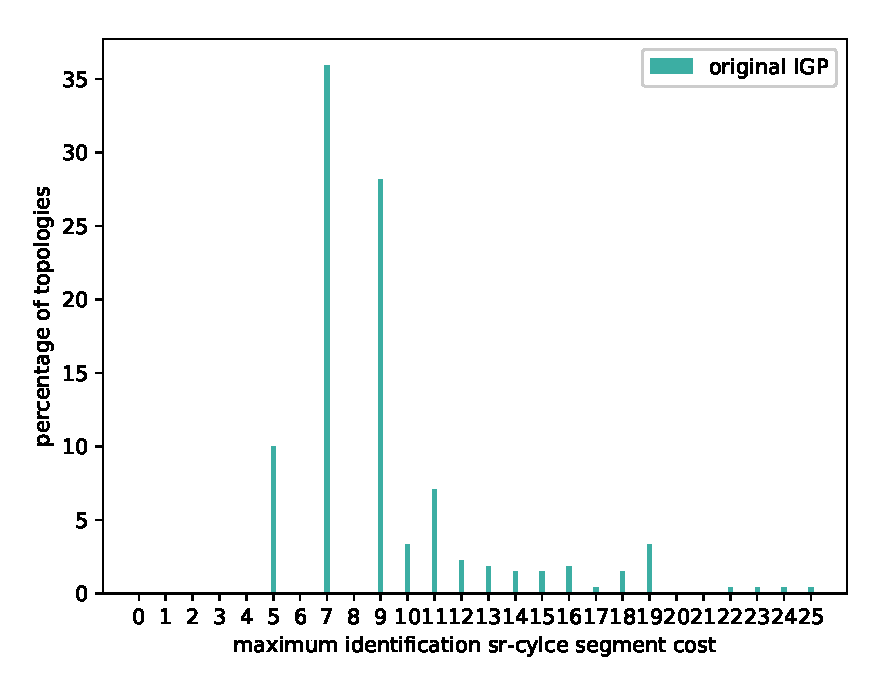
\includegraphics[width=.85\columnwidth]{./Network-lib/data/plot/minSegCover_identification_orig.eps}
\end{center}
\caption{Distribution of the maximum segment cost of the probing sr-cycles.}
\label{fig:min-seg-cost-segcost-orig}
\end{figure}


\begin{algorithm}[t]
\small
\caption{$\textsf{find-faulty-edge}\left( g, \sr{c} = \langle x_1, \ldots, x_l \rangle \right)$}
\begin{algorithmic}[1]
\STATE $c = (e_1, \ldots, e_n) \gets \seq(\sr{c})$
\STATE $L \gets 0, R \gets n$
\WHILE{$R - L \geq 2$}
  \STATE $i \gets \frac{L + R}{2}$
  \IF{$g.\textsf{isSymmetric}()$}
    \STATE $j \gets \min \ \left\{ j \in \{ 1, \ldots, l \} \mid e_i = x_j \vee \left(j < l \wedge e_i \in \sp(x^2_{j}, x^1_{j + 1})\right) \right\}$
    \IF{$e_i = x_j$}
      \STATE $\sr{c}_i \gets \langle x_1, \ldots, x_j, \rev(x_j), \ldots, \rev(x_1) \rangle$
    \ELSE
      \STATE $\sr{c}_i \gets \langle x_1, \ldots, x_{j - 1}, e^2_i, \rev(x_{j - 1}), \ldots, \rev(x_1) \rangle$
    \ENDIF
  \ELSE
    \STATE $\sr{c}_i \gets \textsf{min-segmentation}((e_1, \ldots, e_i, \rev(e_i), \ldots, \rev(e_1))$
  \ENDIF
  \STATE $\textit{status} \gets \textsf{send-probe}(\sr{c}_i)$
  \IF{$\textit{status} = \textit{received}$}
    \STATE $L \gets M$
  \ELSE
    \STATE $R \gets M$
  \ENDIF
\ENDWHILE
\IF{\textit{single-link failures}}
  \RETURN $e_L$
\ENDIF
\RETURN $\{ e_L, \rev(e_L) \}$
\end{algorithmic}
\label{algo:findedge}
\end{algorithm}

% 
% \subsection{Computing the cycle cover}
% 
% 
% \subsection{Min segment cost cycle cover}
% 
% \begin{lemma}
% \label{lemma:deterministic-concat2}
% Let $\sr{p} = \langle x_1 \ldots, x_l \rangle$ be a deterministic sr-path from $u_1$ to $u_2$ and 
% $\sr{q} = \langle y_1, \ldots, y_r \rangle$ be a sr-path from
% $v_1$ to $v_2$ such that $u_2 \neq v_1$ and $v_1 \in \nreach(u_2, 1)$. Then $\sr{p} \oplus \sr{q}$
% is a deterministic sr-path from $u_1$ to $v_2$ with 
% 
% \[ \cost(\sr{p} \oplus \sr{q}) =
%   \begin{cases}
%     \cost(\sr{p}) + \cost(\sr{q}) + 1 & \quad \text{if } y_1 \text{ is a node segment}\\
%     \cost(\sr{p}) + \cost(\sr{q})  & \quad \text{otherwise}
%   \end{cases}
% \]
% \end{lemma}
% 
% \begin{proof}
% The fact that $\sr{p} \oplus \sr{q}$ is deterministic is obvious since both $\sr{p}$ and $\sr{q}$ are deterministic and
% since $v_1 \in \nreach(u_2, 1)$ there is a unique shortest path connecting the last node of $\sr{p}$ to the first node of
% $\sr{q}$. Write $\sr{p} \langle x_1 \ldots, x_l \rangle$ and $\sr{q} = \langle y_1, \ldots, y_r \rangle$. If $y_i$ is a node
% segment, its cost is not included in $\sr{q}$ since it is the ingress node of that sr-path. However, it appears as a segment in 
% $\sr{p} \oplus \sr{q}$ since $u_2 \neq v_1$. Therefore in this case the segment cost in increased by $1$. Otherwise $y_i$ was already
% counted in $\cost(\sr{q})$ so the segment cost is just the sum of both costs. Note that the nature of $x_1$ does not matter as it remains
% the origin of the concatenation of the sr-paths.
% \end{proof}
% 
% \begin{lemma}
% \label{lemma:splitCost}
% Let $\sr{p} = \langle x_1, x_2, \ldots, x_l \rangle$. Then, for all $v \in V(G)$ and $i = 1, \ldots, l$ we have that
% $$
% \cost(\langle u, x_{i + 1}, \ldots, x_l \rangle) = \cost(\sr{p}) - \cost(\langle x_1, \ldots, x_i \rangle)
% $$
% \end{lemma}
% 
% \begin{proof}
% Since $u$ is a node segment, $\cost(\langle u, x_{i + 1}, \ldots, x_l \rangle) = \sum_{k = i + 1}^l \cost(x_k)$.
% On the other hand,
% \begin{align*}
% \cost(\sr{p}) - \cost(\langle x_1, \ldots, x_i \rangle) & = \sum_{k = 1}^l \cost(\sr{p}, x_i) - \sum_{k = 1}^i \cost(\sr{p}, x_i) \\
% & = \sum_{k = i + 1}^l \cost(\sr{p}, x_i) \\
% & = \cost(\langle u, x_{i + 1}, \ldots, x_l \rangle)
% \end{align*}
% \end{proof}
% 
% \begin{lemma}
% \label{lemma:splitCost2}
% Let $\sr{p} = \langle x_1, x_2, \ldots, x_l \rangle$, $i \in \{ 1, \ldots, l - 1 \}$, $k = \cost(\sr{p})$, $k_1 = \cost(\langle x_1, \ldots, x_i \rangle)$ 
% and $k_2 = \cost(\langle x_{i + 1}, \ldots, x_l \rangle)$. Then, 
% \[ k_2 =
%   \begin{cases}
%     k - k_1 - 1 & \quad \text{if } x_{i + 1} \text{ is a node segment}\\
%     k - k_1  & \quad \text{otherwise}
%   \end{cases}
% \]
% \end{lemma}
% 
% \begin{proof}
% We have that
% \begin{align*}
% k_2 & = \cost(\langle x_{i + 1}, \ldots, x_l \rangle) = \sum_{j = i + 1}^l \cost(x_j) \\
% \end{align*}
% If $x_{i + 1}$ is an adjacency segment then
% \end{proof}
% 
% 
% \begin{theorem}
% \label{thm:cyclecover}
% Let $G$ be a network, $s \in V(G)$ and $e \in E(G)$.
% There exists a deterministic sr-cycle $\sr{c}$ from $s$ to $s$ of segment cost at most $k$ covering $e = (u_1, u_2)$ if and only
% there exists $r \in \{0, \ldots, k\}$ such that one of these conditions holds
% \begin{enumerate}
%  \item $(u_1, u_2) \in \ereach(r, s)$ and $v \in \nreach(k - r, u_2)$
%  \item there exists $x \in \nreach(r, s)$ and $y \in \nreach(x, 1)$ such that $e \in \sp(x, y)$ and $s \in \nreach^n(k - r - 1, y)$
%  \item there exists $x \in \nreach(r, s)$ and $y \in \nreach(x, 1)$ such that $e \in \sp(x, y)$ and $s \in \nreach^e(k - r, y)$
% \end{enumerate}
% \end{theorem}
% 
% \begin{proof}
% $(\Rightarrow)$ Suppose that $c = \langle x_1, \ldots, x_l \rangle$ is a deterministic sr-cycle from $s$ to $s$ of segment cost at most $k$ covering $e$.
% Since $c$ covers $e$, there exists the smallest $i$ such that $\langle x_1, \ldots, x_i \rangle$
% covers edge $e$.
% 
% \emph{Case 1:} $x_i = e$: Write $r = \cost(\langle x_1, \ldots, x_i \rangle)$. Then, by Lemma \ref{lemma:splitCost},
% $\langle u_2, x_{i + 1}, \ldots, x_l \rangle$ is a sr-path of cost at most $k - r$ from $u_2$ to
% $s$. Hence $s \in \nreach(k - r, u_2)$.
% 
% \emph{Case 2:} $x_i \neq e$: Then, by choice of $i$, $e$ belongs to the unique shortest path betweeh $x^2_{i - 1}$ and $x^1_{i}$.
% Let $x = x^2_{i - 1}$, $y = x^1_i$ and $r = \cost(\langle x_1, \ldots, x_{i - 1} \rangle)$. 
% Then, since $c$ is deterministic, $x = x^2_{i - 1} \in \nreach(s, r)$ and $y = x^1_i \in \nreach(1, x)$.
% If $x_i$ is a node segment then $\langle x_{i + 1}, \ldots, x_l \rangle$ has cost $k - r - 1$ so $s \in \nreach^n(k - r - 1, y)$.
% Otherwise, $\langle x_{i + 1}, \ldots, x_l \rangle$ has cost $k - r$ so $s \in \nreach^e(k - r, y)$. Since $e \in \sp(x, y)$ we 
% see that either condition $2.$ or $3.$ from the above theorem is satisfied.
% 
% $(\Leftarrow)$ Suppose that there exists $r$ such that $(u_1, u_2) \in \ereach(v, r)$ and $v \in \nreach(u_2, k - r)$.
% There there exists a sr-path $\sr{p}$ from $v$ to $u_2$ covering $e$ of segment cost at most $r$ and 
% a sr-path $\sr{q}$ from $u_2$ to $v$ of segment cost at most $k - r$. By Lemma \ref{lemma:deterministic-concat},
% $\sr{c} = \sr{p} \oplus \sr{q}$ is a deterministic sr-cycle from $v$ to $v$ covering edge $e$ with $\cost(\sr{c}) \leq r + k - r = k$
% 
% Suppose now that there exists $x \in \nreach(v, r)$ and $y \in \nreach(x, 1)$ such that $e \in \sp(x, y)$ and $v \in \nreach(y, k - r)$.
% Then there exists a sr-path $\sr{p}$ from $v$ to $x$ with $\cost(\sr{p}) \leq r$ and a sr-path $\sr{q}$ from $y$ to $v$
% with $\cost(\sr{q}) \leq k - r$. Since $y \in \nreach(x, 1)$, by Lemma \ref{lemma:deterministic-concat2} \todo{this lemma does not exists, concatenation of
% paths not ending in the same node but with unique shoretest path between}, $\sr{c} = \sr{p} \oplus \sr{q}$ is a deterministic sr-cycle
% from $v$ to $v$ with $\cost(\sr{c}) \leq r + k - r = k$. Since $e \in \sp(x, y)$ this cycle covers $e$.
% \end{proof}
